\documentclass{mproj}
\usepackage{graphicx}

\usepackage{url}
\usepackage{fancyvrb}
\usepackage[final]{pdfpages}
\usepackage{times}
\usepackage{gensymb}
% for alternative page numbering use the following package
% and see documentation for commands
%\usepackage{fancyheadings}


% other potentially useful packages
%\uspackage{amssymb,amsmath}
%\usepackage{url}
%\usepackage{fancyvrb}
%\usepackage[final]{pdfpages}

\begin{document}
%%%%%%%%%%%%%%%%%%%%%%%%%%%%%%%%%%%%%%%%%%%%%%%%%%%%%%%%%%%%%%%%%%%
\title{Title of project placed here}
\author{Name of author placed here}
\date{Date of submission placed here}
\maketitle
%%%%%%%%%%%%%%%%%%%%%%%%%%%%%%%%%%%%%%%%%%%%%%%%%%%%%%%%%%%%%%%%%%%

%%%%%%%%%%%%%%%%%%%%%%%%%%%%%%%%%%%%%%%%%%%%%%%%%%%%%%%%%%%%%%%%%%%
\begin{abstract}
abstract goes here
\end{abstract}
%%%%%%%%%%%%%%%%%%%%%%%%%%%%%%%%%%%%%%%%%%%%%%%%%%%%%%%%%%%%%%%%%%%

%%%%%%%%%%%%%%%%%%%%%%%%%%%%%%%%%%%%%%%%%%%%%%%%%%%%%%%%%%%%%%%%%%%
\educationalconsent

%%%%%%%%%%%%%%%%%%%%%%%%%%%%%%%%%%%%%%%%%%%%%%%%%%%%%%%%%%%%%%%%%%%

\newpage
%%%%%%%%%%%%%%%%%%%%%%%%%%%%%%%%%%%%%%%%%%%%%%%%%%%%%%%%%%%%%%%%%%%
\section*{Acknowledgements}

acknowledgements go here sdfsdf

%%%%%%%%%%%%%%%%%%%%%%%%%%%%%%%%%%%%%%%%%%%%%%%%%%%%%%%%%%%%%%%%%%%
\tableofcontents
%%%%%%%%%%%%%%%%%%%%%%%%%%%%%%%%%%%%%%%%%%%%%%%%%%%%%%%%%%%%%%%%%%%

%%%%%%%%%%%%%%%%%%%%%%%%%%%%%%%%%%%%%%%%%%%%%%%%%%%%%%%%%%%%%%%%%%%
\chapter{Introduction}\label{intro}

\section{Sentence}

I completed a program which allowed a turtlebot to autonomously map an environment using SLAM as well as create an inventory of items found in the environment.


\section{Importance/Context/Motivation}

Mobile robots are becoming more and more affordable and accessible which has allowed developers to take advantage of their applications in many different ways. 

SLAM has it's application in rescue robots which
http://www.aaai.org/Pressroom/Releases/release-02-0910.php
these robots required realtime control and utilised only video streams to identify and rescue people.

This compares to this which utilises rugged mobile robots to create SLAM maps of mine shafts with minimal supersvision. This can then be applied to areas which are too unsafe/ small for humans to access.
https://miningrox.informatik.tu-freiberg.de/en/

More affordable Drones can also be used to increasingly accurate create maps of property as well

Object detection can be used to detect humans via heat sensors etc. Aswell as identifying bombs etc.



\section{Objectives/Hypothesis Karl Popper/Problem statement}

\section{Description of Objectives}

\section{How I achieved it} 

\subsection{System Diagram} 

\section{Outline of the dissertation} 




%%%%%%%%%%%%%%%%%%%%%%%%%%%%%%%%%%%%%%%%%%%%%%%%%%%%%%%%%%%%%%%%%%%
\chapter{Background}\label{survey}

This chapter provides research into the hardware and software required to run the Turtlebot and perform autonomous SLAM mapping.
It will consider the processes of object detection and recognition by first considered them in the context of natural visual systems and then in application in software.

\section{Mobile Robots}


Mobile robots are robots that are not fixed to one location and are capable of moving around their environments. Movement is achieved generally through legs, wheels or tracks but aerial and nautical robots can use propellors. The robot can be controlled through manual-tele operation involving a human driver, line-following which follow visual cues such as painted lines to navigate or autonomously. These robots have many applications in areas such as the military, agriculture, rescue, transport and domestic use and include Unmanned Aerial Vehicles (UAV or commonly drones)and self-driving cars.

\subsection{Turtlebot 2}

The Turtlebot 2 is a part of a series of low cost, open-source mobile robots first developed at Willow Garage by Melonee Wise and Tully Foote in 2010. These robots are intended for educational and research purposes and provide an 'low-barrier-of-entry' platform for development while suitable hardware for SLAM and navigation\cite{turtlebot}. The construction of the robot is very flexible featuring a modular support structure that encourages adding additional hardware but the core of the Turtlebot consists of a Kobuki base, a computer running ROS and some form of camera particularly RGB-D or stereo cameras such as the Xbox Kinect or Zed Camera.

\begin{figure}[h]
  \caption{The Turtlebot used for the project. Featuring a Zed Camera and Lenovo Ideapad Y700.}
  \centering
  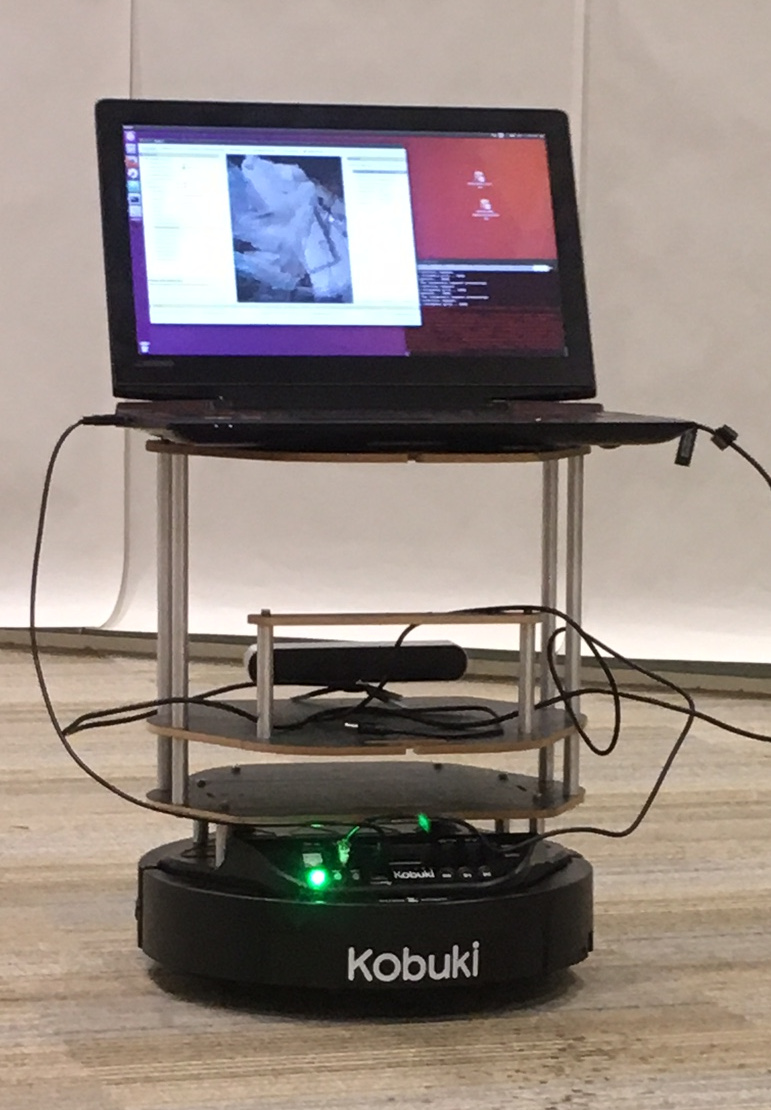
\includegraphics[width=0.5\textwidth]{images/turtlebot.JPG}
  \label{fig:Turtlebot}
\end{figure}
 
The Kobuki base contains sensors and actuators as well as a power supply and vehicular functions. This provides a centralised unit of hardware that can be accessed via the Robot Operating System (ROS). This means that hardware processes are sufficiently abstracted as to be approachable for software developers and other high-level users without an engineering or robotics background. The base has cliff, wheel drop and bumper sensors as well as a gyroscope and highly accurate odometry. 

As it requires a computer running ROS to communicate with, a laptop can simply be attached to the top of the base connected by a USB cable. However, in some cases it may be more convienent to attach a small netbook or Raspberry Pi to the base and then use a seperate computer to remotely communicate with the host machine. The Turtlebot has many bespoke packages for use within ROS, these include standard applications such as teleoperation or navigation and more specialized packages such as frontier exploration. 


\subsection{Cameras}
For nearly all use cases, the Turtlebot requires the use of a camera. While this can be something as simple as a webcam a greater number of applications can be created for it with some form of depth or range measurement received from RGB-D and stereo cameras. Both the discussed cameras are commonly used in ROS and for the Turtlebot.

The Kinect is a very affordable RGB-D camera developed for use on machines running Microsoft Windows though open-source drivers exist for other operating systems. The Kinect is an active camera which utilises a time-of-flight sensor to estimate the distance of points in the field of view. The Zed Camera is a stereo camera with a very user-friendly SDK and wide driver support. 

\begin{table}[ht]
\caption{Comparison of the Zed Camera and Xbox Kinect v2}
\centering 
\begin{tabular}{c | c | c | c}
\hline
 Feature     & Kinect         & Zed Camera \\
 \hline
 Resolution  & 1080p at 30fps & 1080p at 30fps \\
 Depth range & 0.5 - 8m       & 0.5 - 20m \\
 FOV         & 70\degree horz. and 60\degree vert. & 110\degree \\
 Power       & 12V Adapter	  & 5V USB \\			  
\hline
\end{tabular}
\label{table:camera comparison}
\end{table}

\section{Robot Operating System (ROS)}

ROS is a meta-operating system which provides a collection of tools and conventions to aid the writing of robot software. This includes an abstraction of hardware and communications as well as many tools for tasks such as message passing and package management.

ROS features open-source licenses and a large growing collection of packages which contribute to a vibrant ecosystem of developers and researchers working on applications. Some of these packages provide frameworks and algorithms for areas such SLAM and kinematics as well as useful visual and modelling tools. These include:

\begin{itemize}
  \item \textbf{RViz} - a visualisation tool which provides 3D visualisations of sensor data and robot states, such as cameras, lasers and joint states.
 \item \textbf{Gazebo} - a modelling tool which provides a simulated environment to build and test applications in ROS complete with robot sensors and accurate physics.
\end{itemize}


The software engineering principles of loose coupling and abstraction are encouraged throughout design which simplifies software integration and reuse as well as meaning that ROS is generally independent of hardware specifics. ROS features standard implementations in popular programming languages such as Python and C++ which has further increased the community of users.

\subsection{How does ROS work?}

ROS consists of some key components within the communications infrastructure.
\begin{itemize}
  \item \textbf{Nodes} are modular processes performing computation which can communicate with each other using topics or services. A system may consist of many nodes which perform many different tasks.
  \item \textbf{Topics} are named buses which provide a clear message passing interface between nodes. This is achieved through an anonymous publish/subscribe mechanism that allows many-to-many transport.
  \item \textbf{Messages} are a data structure which are published by nodes to topics. They support strongly typed fields such as primitives or arrays and are either predefined or user-defined.
  \item The ROS core or \textbf{Master} provides a centralized node which locates and negotiates communications between nodes as well providing naming and registration services.
  \item \textbf{Services} forgo the many-to-many paradigm and provide a request/reply interaction via servers and clients.
\end{itemize}

\begin{figure}[h]
  \caption{Illustration of general ROS communication concepts}
  \centering
  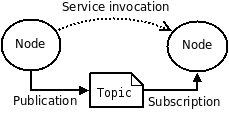
\includegraphics[width=0.5\textwidth]{images/ROS_basic_concepts.png}
  \label{fig:ROS diagram}
\end{figure}

* DIAGRAM OF DESCRIBED SYSTEM

For example a simple robot vehicle system can consist of three nodes. The first node controls the robot's ultrasonic range finder and is publishing a stream of range messages taken from the sensor along the \texttt{sensor/sonar} topic.

The second node controls the robot's movement hardware and is publishing the robot's orientation on the \texttt{geometry\char`_msgs/pose} topic. It also contains an actionlib server which responses to requests to change the robot's positioning. 

The third node controls the robot's movement and is subscribed to the \texttt{sensor/sonar} topic and contains a client of the actionlib server. While processing the range messages, if the range indicated is very small the node can use the actionlib service to request an adjustment in the orientation of the robot thus meaning the robot will avoid collisions. 



\section{SLAM (Simultaneous Localisation and Mapping)}

SLAM is the problem of simultaneously localising (finding the pose and orientation) of a camera within it's surroundings at the same time as mapping the structure of the environment. This requires a robot or camera with the ability to produce odometry readings as well as a camera with a range measurement device.

SLAM forms the basis of navigation in most mobile robots, meaning unknown environments can be explored and mapped without the need for technology such as GPS which is not precise. It has applications in a range of manned and autonomous robots. This includes UAVs, underwater robots and domestic robots such automatic lawnmowers. SLAM is also a key component in the development of self-driving cars These cars are driven along routes while performing SLAM capturing location, feature and obstacle data. Once the map is completed it is processed and the cars are driven autonomously along these routes updating the map as necessary.


\begin{figure}[h]
  \caption{Illustration of the SLAM problem.}
  \centering
  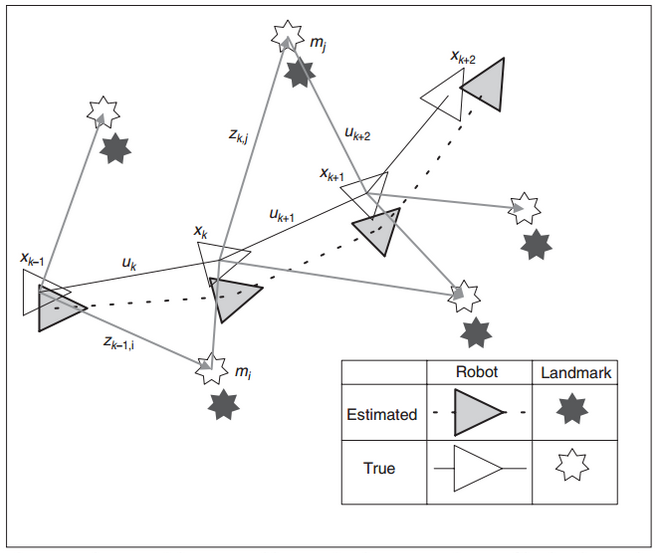
\includegraphics[width=0.5\textwidth]{images/slam_problem.png}
  \label{fig:SLAM Problem}
\end{figure}
https://blog.acolyer.org/2015/11/05/simultaneous-localization-and-mapping-part-i-history-of-the-slam-problem/

This is considered to be a solved problem in Computer Science and their are many different approaches for finding a solution \cite{Hugh2006}. But at a high level SLAM is solved by using the environment to update the pose of the robot. Using odometry as the sole measurement of localisation has an element of uncertainity due to extraneous factors such as wheels slipping on different environments meaning that a stated distance given by an odometry reading may be over or under estimated. 

Therefore laser scans or other forms of depth readings are used to correct the robot's position by extracting features from the surrounding environment. These are called landmarks and can be extracted by various methods such as Random Sampling Consensus (RANSAC) and provide a growing map of the enviroment. Recognising previously visited landmarks is process known as loop closure detection where matches are found between new observations  and regions of the map determined by the uncertainty associated  with the robot’s position\cite{labbe13appearance}.

Most SLAM solutions are probalistic and for example, can use a Kalman to track the uncertanity of the robot within the map using erroneous range observations and robot controls such as odometry over time. Formally:

\[ \textit{P}\left(x, m | z_{1:t}, u_{1:t}\right) \]

Where:

Given:

Robot controls $ u_{1:t} = \lbrace u_{1}, u_{2}, u_{3} ... u_{t} \rbrace $

Observations $ z_{1:t} = \lbrace z_{1}, z_{2}, z_{3} ... z_{t} \rbrace $

Wanted:

Map of the Environment $ m $

Path of the robot $ x_{0:t} = \lbrace x_{1}, x_{2}, x_{3} ... x_{t} \rbrace $

(Starts at 0 to fix a coordinate frame)


SLAM was considered an especially difficult problem to solve \cite{Hugh1988} because these variables cannot be fully decoupled as can be observed in Figure []???. For example a map is required for localising landmarks  which requires pose estimates.

\begin{figure}[h]
  \caption{Graph illustrating the dependencies between SLAM variables.}
  \centering
  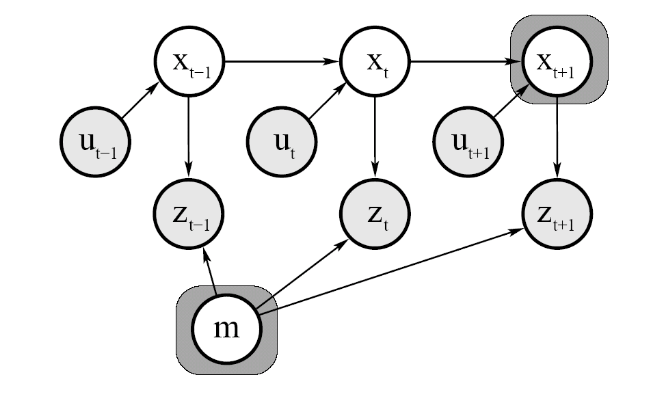
\includegraphics[width=0.5\textwidth]{images/slam_graph.png}
  \label{fig:SLAM Graph}
\end{figure}


\subsection{RTABMap}

ROS features many different applications of SLAM including a popular wrapper for OpenSlam's Gmapping which produces a 2D occupational grid map.\cite{gmapping} Another approach is RTABmap (Real-Time Appearance-Based Mapping) which produces a 3D point cloud map as well as 2D occupancy grid map. It is a RGB-D Graph-Based approach based on an incremental appearance-based loop closure detector. 

\begin{figure}[h]
  \caption{Graph  representation  of  locations.  Vertical  arrows  are  loop  closure
links and horizontal arrows are neighbour links. Dotted links show not detected
loop closures. Black locations are those in LTM, white ones are in WM and
gray ones are in STM. Node 455 is the current acquired location}
  \centering
  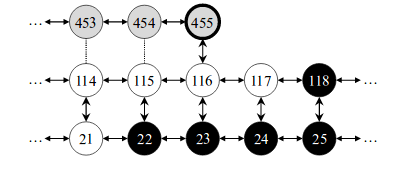
\includegraphics[width=0.5\textwidth]{images/graph.png}
  \label{fig:RTABMap Graph diagram}
\end{figure}

In most probablistic SLAM approaches loop closure detection compares newly found landmarks to previously visited landmarks. This takes an exponential amount of time as the time required to process new landmarks increases with the number of visited landmarks found on the map. A delay is introduced if this process is greater than the time it takes to find a new landmark thus deteriorating the accuracy of the map produced.
 
\begin{figure}[h]
  \caption{RTAB-Map memory management model.}
  \centering
  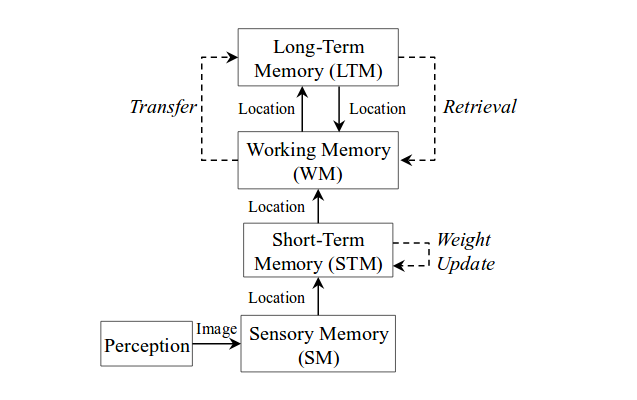
\includegraphics[width=0.5\textwidth]{images/memory.png}
  \label{fig:RTABMap Memory diagram}
\end{figure}

RTAB-Map uses an efficient memory management technique to minimise this problem by keeping the most frequent and recently observed landmarks in the robot's Working Memory (WM) and transfers the others into a Long-Term Memory(LTM). \cite{labbe13appearance} Locations in LTM are not used for loop closure detection and thus a weighting system using a graph of landmarks is used. When  landmarks need to be transfered from  WM to LTM the landmark with the lowest weight is selected. 


\section{Object Detection and Classification}

\subsection{Introduction}
Object detection is the task of finding the potential real-world objects within images or videos while classification involves giving these objects the correct label. Alongside robotics, such technology has applications in areas such as surveillance, medical image analysis and human computer interaction. Modelling a intelligent agent that interprets objects in scenes can be modelled on natural visual systems as many organism's vision systems have much less resolution, sensitivity and field of vision than a modern camera yet are able to perform incredibly complex tasks successfully. 

It is useful to think of object detection software in terms of an intelligent agent which is an autonomous entity that gathers and observers information through sensors and acts upon an environment using actuators to direct its activity to achieve goals.\cite{Norvig2003} Why???


\subsection{Detection in the Natural World}

For most visual systems while everything is seen for the first time our senses do not keep telling us things we already know, this is because between scenes, most important environmental information stays constant. This process is a form of sensory adaption where perception is temporarily changed when exposed to new stimuli in an attempt to normalise visual experience.\cite{Webster2015} This happens at a retinal and neural level, where information provided by past experience have a greater say on how a scene has been interpreted than immediate information provided by external organs. 

For example an ellipse projected into a human retina can be interpreted as a circle due to our experiences with perspective. 
%\cite{The eye the brain the computer p208}

Many species exhibit a form of pattern or feature detection to trigger neural responses to visual changes. In contrast to humans which detect generic images features such as shapes, many lower organisms utilise goal-based feature detection. This is useful to the field of computer science because it allows us to model intelligence agents on such processes, which are typically simple and linear in that there is only one way of achieving the goal and that task assumes the agents complete engagement.

For example arthopods such as honey bees readily distinguish features such as flowers in the environment that pertain to the goal of gathering food. Similarly a frog's eye is stimulated when a black disc moves in an arc rapidly within the receptor field indicating that a flying insect is near and triggers the frogs feeding response \cite{} thus satisfying the goal of feeding.

Once objects have been detected and classified by a creature are they retained in memory...
 
\subsection{Attention Systems - Memory Hierachy}
\subsubsection{Spatial temporal Attention Models}

How long do organism retain visual information.

How spatial temporal reasoning
- don't overload memory
- Have a Buffer
- reaffirm spatial temporal Attention
Memory Hierarchy
- 9 seconds, How long?
- What is long term?
- What is short term? 
- What is important
- How to decide
- Intelligence agents

Humans forget things when they leave a room.
 
\subsection{Extracting Features}

What determines if an area of a scene is worth triggering neural activity is different for different species. In image processing software attempts are made to find features which are unique, that can be easily tracked and can be easily compared. These features can be used for many different types of processing such as calculating a histogram of oriented gradients (HOG) which can then used for object classifiers.

\subsubsection{FAST Feature Detection}

There are many software applications of feature detection, this includes SIFT (Scale-Invariant Feature Transform) which performs extremely well in most contexts\cite{Mikolajczyk}. However for applications in real-time image processing such as SLAM and Augmented Reality it is often not fast enough. FAST (Features from Accelerated Segment Test) \cite{rosten_2006_machine}\cite{rosten_2005_annotations} avoids the costly difference of Gaussians (DoG) method found in SIFT and is subsequently much faster.

Using an appropriate threshold $T$ which is usually 12, the algorithm selects a pixel $P$ which is the centre of a circle with a circumference of 16 pixels, $n$ and the pixel's $P$ intensity is $I_{p}$. The pixel $P$ is determined to be a corner if $n$ are all brighter than $I_{p} + t$ or are all darker than $I_{p} - t$. 

\begin{figure}[h]
  \caption{Illustration of the FAST}
  \centering
  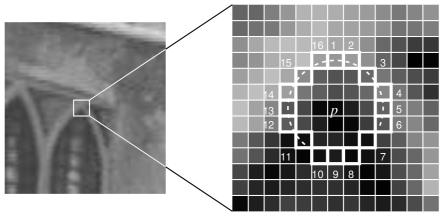
\includegraphics[width=0.5\textwidth]{images/fast_speedtest.jpg}
  \label{fig:FAST diagram}
\end{figure}

If a threshold $T$ of 12 or greater is used a high speed test is performed to reject a large number of non-corner points which involves examining the pixels at 1, 9, 5, 13. If either pixel 1 or 9 are brighter or darker than $T$ then 5 and 13 are checked. Therefore, if three of these pixels are either all darker than the threshold or all brighter then $P$ is determined to be a corner. 

\subsection{Object Classification with Deep Learning}

Determining what an object is is from within an image generally requires a form of  classifier which utilises a training set of identified images and a validation set. One such approach is Deep Learning which is based on the way the human brain processes information and learns. Deep Learning is a form of machine learning that involves feeding data through neural networks composed of many layers. This allows data to be processed in a hierarchical way where each layer recognizes higher or more abstract features than the previous layer.

\begin{figure}[h]
  \caption{Need to add******}
  \centering
  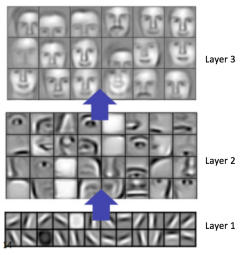
\includegraphics[width=0.5\textwidth]{images/layers.png}
  \label{fig:Deep Net Layers diagram}
\end{figure}


\subsubsection{Convolutional Neural Networks (CNN)}
  
Convolutional Neural Networks (CNN) are a type of deep neural network which since 2012\cite{} has been  increasingly popular and suited for object recognition and classification in images. This is namely because:

\begin{itemize}
\item it is rugged to distortions such as different lighting and  occlusion
\item training can be spread across several GPU's resulting in very deep networks
\item it features fewer parameters than standard neural networks meaning training time is substantially reduced
\end{itemize}

A CNN uses many identical copies of the same neuron, meaning the network can have a large amount of neurons thus expressing computationally large models while keeping the parameters the neurons have to learn very small. \cite{NIPS2012_4824}
  
An approach called \textit{symmetry} is used to look for properties in the data where at each segment of data we care about the same properties at the same time. Therefore a group of neurons, $A$ can be introduced to a neural network that computes certain features such as the presence of an edge and then the output of this layer is fed into a fully-connected layer, $F$. ****Not convincing
  
\begin{figure}[h]
  \caption{The convolutional layer is represented by the group of neurons $A$.}
  \centering
  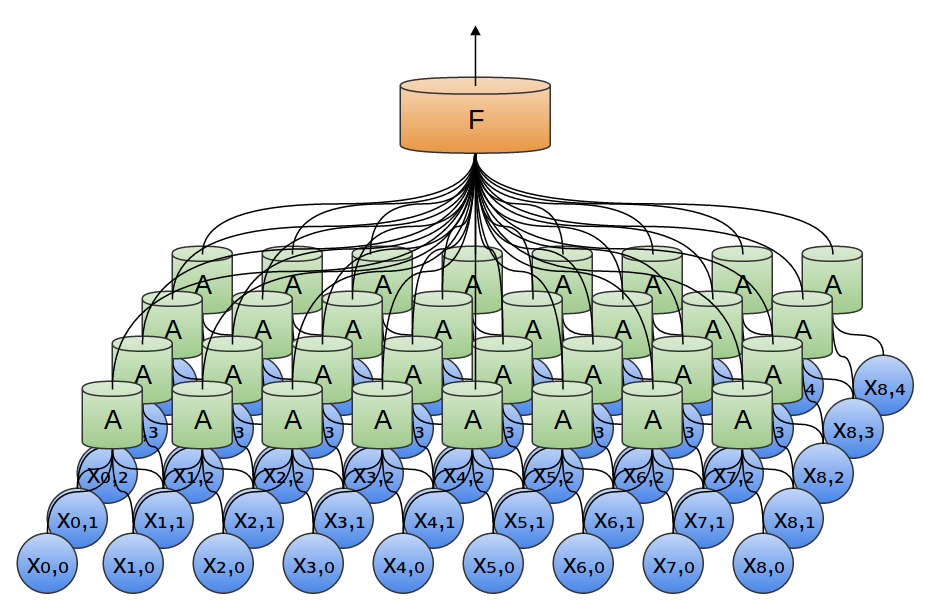
\includegraphics[width=0.5\textwidth]{images/conv.png}
  \label{fig:Basic CNN diagram}
\end{figure}

These convolutional layers are composable, meaning you can feed the output into the input of another layer detecting more abstract features. A max-pooling layer is often used which takes the maximum features over segments of a previous layer, this allows further convultional layers to work on larger sections of the data, this works because it is not wholly useful to know the exact pixel position of an edge but it is enough to know it's location within a few pixels.
 
\begin{figure}[h]
  \caption{Featuring a max-pooling layer}
  \centering
  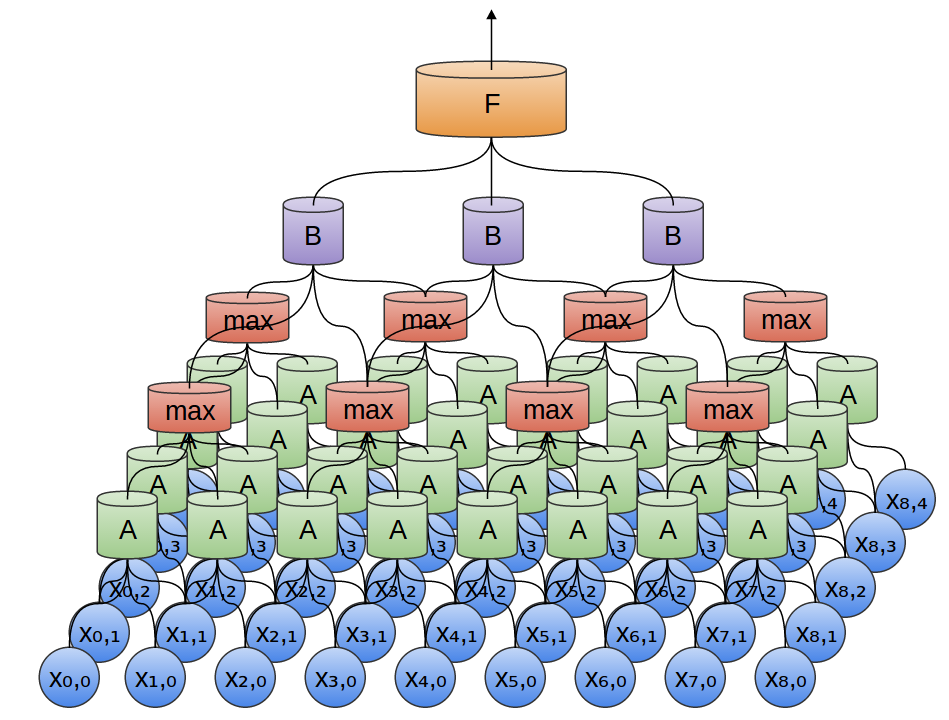
\includegraphics[width=0.5\textwidth]{images/conv_max.png}
  \label{fig:Basic CNN with Max-pooling diagram}
\end{figure}

At every convolution an element-wise operation called Rectified Linear Unit (RelU)is performed that replaces negative pixel values with zeros. This introduces non-linearity into the network because most real world data is linear.

http://colah.github.io/posts/2014-07-Conv-Nets-Modular/

\subsubsection{MobileNet with TensorFlow}
TensorFlow is an open source software library produced by Google Brain for machine learning. It is frequently used due to the fact that it discovers and uses GPUs and multiple cores by default allocating 100\% of GPU RAM for each process, this results in a very high performance. In TensorFlow, computations are represented as a graph, nodes are representations of operations and edges are multi-dimensional arrays called tensors (represented as numpy in Python). This graph occurs within a session and is executed on the CPU or GPU. 
  
MobileNet is a is a deep convolutional neural network for image recognition found in TensorFlow\cite{HowardZCKWWAA17}. The model has been trained on the 2012 ImageNet dataset and is highly optimized for efficiency and size at the expense of accuracy. However the error rate of not providing a correct classification within the top five results is only 10.5\% which for most applications is adequate. Like most pre-trained models it can be retrained to solve specific problems. This network has been used for real-time classifications on memory scarce devices and is particularly applicable to robotics.
  
  \subsubsection{Google Vision API}
  
The Google Vision API is a cloud implementation of a deep convolutional neural networks trained from Google images and implemented with TensorFlow. As part of the Google Cloud platform users can make RESTful API calls from their language of choice querying images to be classified. The service provides label detection and facial detection amongst other features such as SafeSearch which filters images based on their obscene content\cite{googlevision}.

\subsection{Regions with Convolutional Neural Networks (R-CNN)}

Detection systems utilise classifiers to evaluate potential objects. Yet there is no standard way of localising objects within an image which is often in robotics for example to estimate the distance of such object. One such approach is called Regions with Convolutional Neural Networks (R-CNN) and is considerable more efficient than previous approaches and at the time of it's release, R-CNN had the best detection performance on the PASCAL VOC 2012 image dataset. In the paper "Rich Feature Hierarchies For Accurate Object Detection and Semantic Segmentation"\cite{Girshick2014} the authors suggest a method which involves taking an image and identifying objects using bounding boxes and then performing a classification on these areas to create a label for each object. 

\begin{figure}[h]
  \caption{Illustration of the stages found in R-CNN}
  \centering
  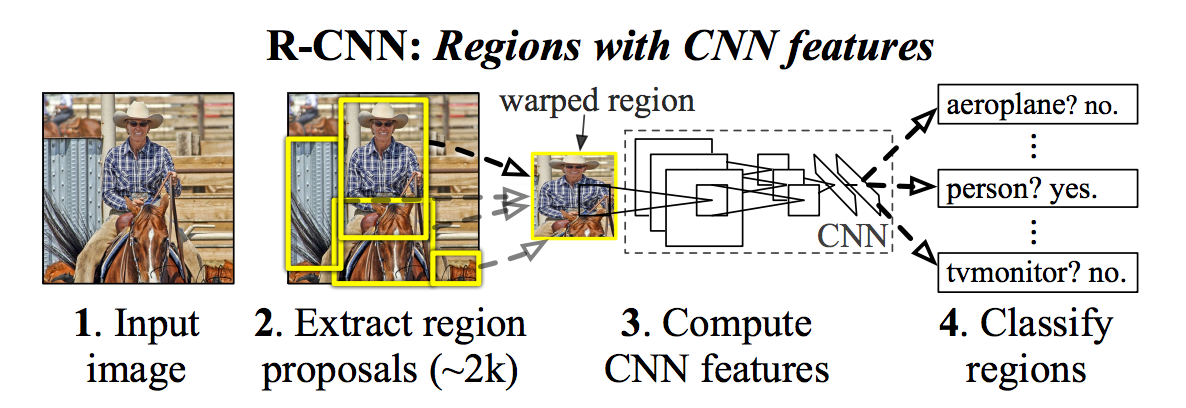
\includegraphics[width=1.0\textwidth]{images/RCNN.png}
  \label{fig:RCNN Diagram}
\end{figure}

Roughly two thousand bounding boxes, or region proposals are created using the process of Selective Search which performs a segmentation algorithm that groups regions together by color, intensity or texture.\cite{Sande2013} This is in contrast to using an exhaustive sliding window approach found in Deformable Parts Models.\cite{voc-release4} Each selected region is warped to a 227 x 227 square RGB image and fed through a CNN which computes features. The final stage involves running a Support Vector Machine (SVM) on the feature vector of each region to classify and score the object within the region (if any). Greedy non-maximum suppression is used to merge the regions which share the same object resulting in accurate bounding boxes for each object. 


\section{Summary and Discussion}
\subsection{What currently exists for completing the objectives}
\subsection{What are the Gaps, What do I have to do to fill the gaps}
\subsection{What methods are not appropriate to fill the gap}




%%%%%%%%%%%%%%%%%%%%%%%%%%%%%%%%%%%%%%%%%%%%%%%%%%%%%%%%%%%%%%%%%%%
\chapter{Approach/Implementation/System Implementation}

\section{Requirements}

Open project - requires stating specific requirements to focus the task
\section{Anaylsis the approaches}

What problems I encounted etc.

\section{Analysis of approaches}
\section{How did I go about it}

\section{Mapping}
\subsection{Transforming data}
\subsection{Calibration}

\section{Frontier Exploration} !!!
Hybrid approach taken from RCNN, currently only has an official matlab binding of RCNN.

Do not use bounding boxes, as not entirely useful in mapping as this requires new detections and classifiations when changing the object pose. A simple spherical location detector is used to show the object is located within the this region of alpha

\section{Object Detection and Recognition}
\subsection{Detecting ROI in FOV}
\subsubsection{Masking}
\subsubsection{Depth Mask}
\subsubsection{HSV Mask}
\subsection{Detecting Objects Clustering - different methods}
\subsection{Creating Boxes with DBScan}
\subsection{Tracking Boxes}
\subsection{Recognising Objects}

Using google vision means that speed does not decreae with more objects detected, statys constant


Transfer learning whereby a pre trained model is retrained for a similar problem.
\subsection{Publishing to Rviz/Rtabmap}
\section{The whole package - how to utilise}

I did this because of that which allows me to do this

%%%%%%%%%%%%%%%%%%%%%%%%%%%%%%%%%%%%%%%%%%%%%%%%%%%%%%%%%%%%%%%%%%%
\chapter{Evaluation}
\section{Testing}
https://www.koen.me/research/pub/vandesande-iccv2011.pdf

Experiment 1
Question
Experiment 2
Experiment 3


I think by doing this I will achieve...
Experiments to answer questions

%%%%%%%%%%%%%%%%%%%%%%%%%%%%%%%%%%%%%%%%%%%%%%%%%%%%%%%%%%%%%%%%%%%
\chapter{Conclusion}\label{conclusion}
\subsection{Future work}

incorporate active detection of features next time.

\appendix % first appendix
%%%%%%%%%%%%%%%%%%%%%%%%%%%%%%%%%%%%%%%%%%%%%%%%%%%%%%%%%%%%%%%%%%%
\chapter{First appendix}

\section{Section of first appendix}

%%%%%%%%%%%%%%%%%%%%%%%%%%%%%%%%%%%%%%%%%%%%%%%%%%%%%%%%%%%%%%%%%%%
\chapter{Second appendix}

%%%%%%%%%%%%%%%%%%%%%%%%%%%%%%%%%%%%%%%%%%%%%%%%%%%%%%%%%%%%%%%%%%%
% it is fine to change the bibliography style if you want
\bibliographystyle{plain}
\bibliography{mproj}
\end{document}
